\documentclass[]{book}
\usepackage{lmodern}
\usepackage{amssymb,amsmath}
\usepackage{ifxetex,ifluatex}
\usepackage{fixltx2e} % provides \textsubscript
\ifnum 0\ifxetex 1\fi\ifluatex 1\fi=0 % if pdftex
  \usepackage[T1]{fontenc}
  \usepackage[utf8]{inputenc}
\else % if luatex or xelatex
  \ifxetex
    \usepackage{mathspec}
  \else
    \usepackage{fontspec}
  \fi
  \defaultfontfeatures{Ligatures=TeX,Scale=MatchLowercase}
\fi
% use upquote if available, for straight quotes in verbatim environments
\IfFileExists{upquote.sty}{\usepackage{upquote}}{}
% use microtype if available
\IfFileExists{microtype.sty}{%
\usepackage[]{microtype}
\UseMicrotypeSet[protrusion]{basicmath} % disable protrusion for tt fonts
}{}
\PassOptionsToPackage{hyphens}{url} % url is loaded by hyperref
\usepackage[unicode=true]{hyperref}
\hypersetup{
            pdftitle={Seed Manual},
            pdfauthor={Deependra Dhakal},
            pdfborder={0 0 0},
            breaklinks=true}
\urlstyle{same}  % don't use monospace font for urls
\usepackage{natbib}
\bibliographystyle{apalike}
\usepackage{longtable,booktabs}
% Fix footnotes in tables (requires footnote package)
\IfFileExists{footnote.sty}{\usepackage{footnote}\makesavenoteenv{long table}}{}
\usepackage{graphicx,grffile}
\makeatletter
\def\maxwidth{\ifdim\Gin@nat@width>\linewidth\linewidth\else\Gin@nat@width\fi}
\def\maxheight{\ifdim\Gin@nat@height>\textheight\textheight\else\Gin@nat@height\fi}
\makeatother
% Scale images if necessary, so that they will not overflow the page
% margins by default, and it is still possible to overwrite the defaults
% using explicit options in \includegraphics[width, height, ...]{}
\setkeys{Gin}{width=\maxwidth,height=\maxheight,keepaspectratio}
\IfFileExists{parskip.sty}{%
\usepackage{parskip}
}{% else
\setlength{\parindent}{0pt}
\setlength{\parskip}{6pt plus 2pt minus 1pt}
}
\setlength{\emergencystretch}{3em}  % prevent overfull lines
\providecommand{\tightlist}{%
  \setlength{\itemsep}{0pt}\setlength{\parskip}{0pt}}
\setcounter{secnumdepth}{5}
% Redefines (sub)paragraphs to behave more like sections
\ifx\paragraph\undefined\else
\let\oldparagraph\paragraph
\renewcommand{\paragraph}[1]{\oldparagraph{#1}\mbox{}}
\fi
\ifx\subparagraph\undefined\else
\let\oldsubparagraph\subparagraph
\renewcommand{\subparagraph}[1]{\oldsubparagraph{#1}\mbox{}}
\fi

% set default figure placement to htbp
\makeatletter
\def\fps@figure{htbp}
\makeatother

\usepackage{booktabs}

\usepackage{geometry} % for custom layout of book and landscape geometry support
\usepackage{amsthm}
\makeatletter
\def\thm@space@setup{%
  \thm@preskip=8pt plus 2pt minus 4pt
  \thm@postskip=\thm@preskip
}
\makeatother

\usepackage{longtable}
\usepackage{booktabs}
\usepackage{dcolumn}
\usepackage{tabularx}
\usepackage{array}
\usepackage{multirow}
% \usepackage[table]{xcolor}
\usepackage{wrapfig}
\usepackage{float}
\usepackage{colortbl}
\usepackage{pdflscape}
\usepackage{tabu}
\usepackage{threeparttable}
\usepackage[normalem]{ulem}
\usepackage{rotating}
\newcommand{\blandscape}{\begin{landscape}}
\newcommand{\elandscape}{\end{landscape}}
\usepackage[format=hang,labelfont=bf,margin=0.5cm,justification=centering]{caption}
% \usepackage{exam} % this and exam.sty cause error
\usepackage{pdfpages}

% \usepackage{subcaption} % doesn't work with tinytex in windows
% \newcommand{\subfloat}[2][need a sub-caption]{\subcaptionbox{#1}{#2}}

% simple fix for exam class features of questions and solution
\usepackage{enumitem}

\newlist{questions}{enumerate}{3}
\setlist[questions]{label=\arabic*.}
\newcommand{\question}{\item}

\newenvironment{solution}{ {\bfseries Solution}:}{}
% \usepackage[latin1]{inputenc}
\usepackage{tikz}

\usepackage{siunitx}
\usepackage{fancyhdr}
\usepackage{etoolbox}
\makeatletter
\providecommand{\subtitle}[1]{% add subtitle to \maketitle
  \apptocmd{\@title}{\par {\large #1 \par}}{}{}
}
\makeatother

\title{Seed Manual}
\providecommand{\subtitle}[1]{}
\subtitle{Standard Operating Procedure}
\author{Deependra Dhakal}
\date{2021-06-27}

\begin{document}
\maketitle

{
\setcounter{tocdepth}{1}
\tableofcontents
}
\chapter{Administrative System}\label{adminsys}

\section{Scope and Purpose}\label{scope-and-purpose}

The administrative division is the main support unit among all remaining
technical units of CSTL. It provides human resources along with material
and financial aid to all divisions and units of the organization. In
coupled with them it provides secretarial services, staff management,
store facilities, procurement as well as repair and maintenance of the
equipment and other machineries.

Seed samples are submitted to Sample Reception Unit of Administration
Division along with the official request letter and are registered here.

\section{Procedure}\label{procedure}

\begin{enumerate}
\def\labelenumi{\arabic{enumi}.}
\tightlist
\item
  Each sample along with all the set of Forms that has been prepared in
  the sample reception area is passed on to the Chief of Administration
  Division.
\item
  The chief of the Division examines the sample and the request letter.
  If the client has provided required information adequate quantity of
  the seed sample, the client will not be made to provide further
  clarification otherwise the clear information is generally sought
  before proceeding. The sample is coded and distributed along with the
  respective forms to the concerned laboratory unit or units for
  requested test data.
\item
  The covering letter accompanied with the submitted sample is retained
  with the administration unit in a covered folder.
\item
  The laboratory units, on the other hand, submit the test results with
  checking by units in- charge to the administration unit as soon as the
  forms/ cards have been duly filled with the test results and comments.
  The administration unit files them in the respective folder for
  further action.
\item
  Results are reported in the percentage and recalculation is done if
  necessary. Such recalculations are generally carried in the respective
  laboratory unit.
\item
  The purity test results are generally converted into percentage by
  weight. The duplicate percentages are averaged and checked against the
  respective tolerance tables. It, they are not in consistent with the
  tolerance level, additional duplicate tests are performed.
\item
  Germination test results are expressed in percentage by weight based
  on number of seeds. If the result is found to be out of tolerance
  level, the administration division asks the germination laboratory
  unit to repeat the tests by providing a new set of Pure Seed and Seed
  Analysis Card (Annex-I)
\item
  As soon as all data are furnished with the aid of concerned
  laboratories, a final check is made for the completeness and
  correctness of data and only then the test result or the test
  certificate in the Standard Report Format (Annex-II) is dispatched to
  the client.
\item
  A copy of the report along with all other relevant analysis cards are
  filed in the respective cover and is stored in a filing cabinet under
  ``completed tests''. These test results are preserved at least for a
  season or for a period as required under Seed Act and Rules before
  they are disposed off.
\item
  The administration unit does also take the responsibility of duly
  maintenance and servicing of the testing equipment and quality
  management system of the laboratory unit.
\item
  The administration unit offers a best possible service to the client
  and looks for to avail the results to the client whenever requested.
\item
  For the smooth and effective operation of the laboratory, proper
  routing of the sample from the registration through reporting becomes
  very important and prevailing flow diagram is attached.
\end{enumerate}

\hypertarget{htmlwidget-2596c05ed408b554c595}{}

\chapter{Seed Sampling}\label{seed-sampling}

\section{Scope}\label{scope}

Various attributes of seed such as analytic, physiological, pathological
and to some extent variety characteristics are determined in the
laboratory based on different tests. Such determinations can only be an
estimate unless the whole quantity of seed lot is tested. This is
practically impossible, as a lot usually contains a large quantity of
seed. Under such circumstances, to give as accurate an estimate as
possible representative samples are prepared.

A composite sample is obtained from the seed lot by drawing out small
portions at random from different positions in the lot and thoroughly
mixing them together. At each stage, thorough mixing is followed either
by progressive sub-division or by the abstraction and combination of
small portions at random.

\section{Object}\label{object}

The objective of sampling is to obtain a sample of a size suitable for
tests, in which probability of a constituent being present is determined
only by its level of occurrence in the seed lot.

\section{Definitions}\label{definitions}

\subsection{Seed Lot}\label{seed-lot}

A Seed lot is a specified quantity of seed that is physically and
uniquely identifiable.

\subsection{Primary Sample}\label{primary-sample}

A primary sample is a small portion taken from the seed lot during one
single sampling action.

\subsection{Composite Sample}\label{composite-sample}

The composite sample is formed by combining and mixing all the primary
samples to taken from the lot.

\subsection{Working Sample}\label{working-sample}

The working sample is a sub-sample taken from the submitted sample in
the laboratory, or a sub-sample thereof, on which one of the quality
tests described in these ISTA Rules is made and must be at least the
weight prescribed by the ISTA Rules for the particular test.

\subsection{Submitted Sample}\label{submitted-sample}

A submitted sample is a sample that is to be submitted to the testing
laboratory and may comprise either the whole of the composite sample or
a subsample thereof. The submitted sample may be divided into subsamples
packed in different material meeting conditions for specific tests
e.g.~moisture or health.

\subsection{Duplicate sample}\label{duplicate-sample}

A duplicate sample is another sample obtained for submission from the
sample composite and marked `Duplicate sample'.

\subsection{Sub-sample}\label{sub-sample}

A submitted sample is a portion of a obtained by reducing a sample.

\subsection{Sealed}\label{sealed}

Sealed means that the containers or individual container in which the
seed is held are closed in such a way that, it cannot be opened to gain
access to the seed and closed again, without either destroying the seal
or leaving evidence of tempering. This definition refers to the sealing
of seed lots, as well as of seed samples.

\subsection{Self-sealing containers}\label{self-sealing-containers}

The `valve-pack' bag is a specific type of self-sealing container. It is
filled through a sleeve-shaped valve which is automatically closed by
the completion of filling the bag.

\subsection{Marked/labeled}\label{markedlabeled}

A container of a seed lot can be considered as marked or labeled when
there is a unique identification mark on the container, which defines
the seed lot to which the container belongs. All containers of a seed
lot must be marked with the same unique seed lot designation (numbers,
characters or combination of both). Marking of samples and sub-samples
must ensure that there is always an unambiguous link between the seed
lot and the samples and sub-samples.

\subsection{Treated seed}\label{treated-seed}

`Seed treatment' is a generic term which indicates that a seed lot has
been subjected to;

\begin{enumerate}
\def\labelenumi{\alph{enumi})}
\item
  the application of a compound including chemicals, nutrients or
  hormones
\item
  the application of a biological product including micro-organisms,
\item
  a process including wetting and drying
\item
  an energy form including heat, radiation, electricity or magnetism but
  does not specify the application method.
\end{enumerate}

Seed treatment does not significantly change the size, shape or add to
the weight of the seeds in the lot.

\section{Conditions for issuing Orange International Seed Lot
Certificates}\label{conditions-for-issuing-orange-international-seed-lot-certificates}

The sampling methods laid down in the ISTA Rules must be followed when
seed samples are drawn for the issue of Orange International
Certificates. Further conditions have to be fulfilled as listed below.

\subsection{Seed lot size}\label{seed-lot-size}

The seed lot must not exceed the quantity indicated in ISTA Rules (Table
2C)

\subsection{Large herbage seed lots of
Poaceae}\label{large-herbage-seed-lots-of-poaceae}

Seeds may have a maximum size of 25000 Kg (with a 5\% tolerance)

\subsection{Check sampling and
testing}\label{check-sampling-and-testing}

After approval, the large seed lots of a production plant must be
monitored by check sampling and further heterogeneity testing and as a
minimum based on purity and other seed count.

If more than one of the last six consecutive check samples tested shows
significant heterogeneity, approval must be withdrawn for the species or
species of group and company must be re-apply for approval.

\subsection{Responsibility}\label{responsibility}

The Seed Quality Control Center in a country is responsible for;

\begin{itemize}
\tightlist
\item
  the decision of approval of the seed company ,
\item
  ensuring that each production plant is approved separately, if a seed
  company has more the one production plant,
\item
  ensuring that testing is done by an ISTA-accredited laboratory,
\item
  the check sampling program.
\end{itemize}

\subsection{Marking /labeling and sealing of
containers}\label{marking-labeling-and-sealing-of-containers}

The seed lot must be in marked/labeled containers which are sealed or
under the control of seed sampler.

Where the seed lot is already marked/labeled and sealed before sampling,
the seed sampler must verify marking /labeling and sealing on every
container. Otherwise the sampler has to mark/label the containers before
seed lot leaves his/her control.

The samplers are personally responsible for seals, labels and bags
supplied to them and it is their duty to ensure that primary, composite
or submitted samples must never be left in the hands of persons not
authorized by the seed testing unless they are sealed in such a way they
cannot be tampered with.

\subsection{Sampling from the seed
lot}\label{sampling-from-the-seed-lot}

Sampling form (Annex-IV) the seed lot methods must be used. An orange
International Seed Lot Certificate issued on a seed lot is still valid
after re-packing the seed lot in new containers provided that,

\begin{enumerate}
\def\labelenumi{\alph{enumi})}
\item
  the identity of the seed in the initial seed lot is preserved
\item
  the seed lot designation is not changed.
\item
  the moving the seed into the new containers is done under the control
  of an ISTA seed sampler.
\item
  there is no processing of the seed during filling of the new
  containers.
\end{enumerate}

\subsection{Submitted sample}\label{submitted-sample-1}

The minimum sizes of submitted samples are as follows

\begin{enumerate}
\def\labelenumi{\alph{enumi})}
\tightlist
\item
  For moisture determination,
\end{enumerate}

100 g for species that must be ground and 50 g for all other species.
When moisture meters are to be used for testing, a large sample size may
be necessary.

\begin{enumerate}
\def\labelenumi{\alph{enumi})}
\setcounter{enumi}{1}
\item
  For verification of species and variety
\item
  For all other test, at least the weight as described in ISTA Rule.
\end{enumerate}

\subsection{Uniformity of the Lot}\label{uniformity-of-the-lot}

At the time of sampling the lot should have been subjected to
appropriate mixing, blending and processing techniques so that it is as
uniform as practicable.

\subsection{Containers}\label{containers}

The lot should be in containers which are sealed in jute bags, metal
drum that are sealed or air tight.

\subsection{Marking and Sealing the
Lot}\label{marking-and-sealing-the-lot}

At the time of sampling, all containers must be sealed, labeled or
marked to show lot identification.

\section{Procedures for Sampling the
Lot}\label{procedures-for-sampling-the-lot}

Sampling is done in two stages:

\begin{enumerate}
\def\labelenumi{\arabic{enumi}.}
\tightlist
\item
  A submitted sample is taken in the warehouse of field and sent to the
  seed-testing laboratory. This sample is usually ten times bigger than
  the quantity required for testing.
\item
  A working sample is prepared from the submitted sample in the
  laboratory for quality test.
\item
  Before the warehouse sampling, the seed lot shall be so arranged that
  each individual container of the lot is conveniently accessible. If
  the nature of the stacking of the lot or type of the container makes
  it impossible to apply procedures adequately, this sampling shall not
  be undertaken and when there is definite evidence of heterogeneity
  either physical or documentary, sampling shall be refused.
\end{enumerate}

\section{Sampling Intensity}\label{sampling-intensity}

\subsection{General principles}\label{general-principles}

The number of primary samples to be taken depends on the size of a lot
and type of containers. A composite sample is obtained from the seed lot
by taking primary samples from different positions in the whole seed lot
and combining them. From this composite sample, four subsamples are
obtained by sample reduction procedures at one or more stages forming
the submitted sample and finally the working samples for testing. For
issuing ISTA Certifications, specific requirements have to be fulfilled.

\subsection{Apparatus}\label{apparatus}

Sampling and sample reduction must be performed using appropriate
techniques and equipment that is clean and in good condition. Containers
(metal) used to collect primary samples, composite sample and during
mixing and dividing must be static free to avoid chaff or small seeds
adhering to the inside of the containers.

\subsection{Procedures}\label{procedures}

\begin{enumerate}
\def\labelenumi{\arabic{enumi}.}
\tightlist
\item
  Procedures for sampling a seed lot
\end{enumerate}

1.1 Preparation of a seed lot and conditions for sampling

At the time of sampling, the seed lot must be as uniform as practicable.
If the seed lot is found to be obviously heterogeneous, sampling must be
refused or stopped. In cases of doubt heterogeneity can be determined.

Seed may be sampled in containers or when it enters containers. The
containers must be fit for purpose, i.e.~must not damage the seed, and
must be clean to avoid cross contamination. The containers must be
labeled or marked before or just after sampling is completed. The seed
lot must be so arranged that each part of the seed lot is conveniently
accessible.

\subsection{Sampling intensity}\label{sampling-intensity-1}

A. For seed lot in containers of 15 kg to 100 kg capacity (inclusively),
the sampling intensity according to Table 2A must be regarded as the
minimum requirements.

B. For seed lots in containers smaller than 15 kg capacity, containers
must be combined into sampling units not exceeding 100 kg, e.g.~20
containers of 5 kg, 33 containers of 3 kg or 100 containers of 1 kg. For
seed mats and tapes, small packets or reels may be combined to sampling
units of not exceeding 2,000,000 seeds. The sampling units must be
regarded containers as in Table 2A.

When sampling seed in containers of more than 100 kg, or from streams of
seed entering containers, the sampling intensity according Table 2B must
be regarded as the minimum requirement.

When sampling a seed lot of up to 15 containers, regard less of their
size, the same number of primary samples must be taken from each
container.

\section{Sampling Instruments and
Methods}\label{sampling-instruments-and-methods}

\subsection{Taking primary samples}\label{taking-primary-samples}

When defining the number and/or the size of primary samples, the seed
sampler needs to ensure (besides meeting the minimum sampling intensity)
that the minimum amount of seed required for the requested test(s) is
sent to the testing laboratory and enough seed remains available for
obtaining duplicate samples if requested.

Primary sample of approximately equal size must be taken from a seed
lot, irrespective of where in the lot or container the primary sample is
taken.

When the seed lot is in containers, the containers to be sampled must be
selected at random or according to a systemic plan throughout the seed
lot. Primary samples must be drawn from the top, middle and bottom of
containers, but not necessarily from more than one position in any
container, unless so specified in Table 2A and Table 2B.

When the seed is in bulk or in large containers, the primary samples
must be drawn from random position. Containers must be opened or pierced
for abstraction of primary samples. The sampled containers must then be
closed or the contents transferred to new containers. When seed is to be
packed in special types of containers (e.g.~small, not penetrable, or
moisture-proof containers), it should be sampled, if possible, either
before or during the filling of the containers.

The instruments being used must neither damage the seed nor select
according to seed size, shape, density, chaffiness or any other quality
trait. All sampling apparatus must be clean before use to prevent cross
contamination. Trier must be long enough so that the opening at the tip
reaches at least half of the diameter of the container. When the
container is not accessible from opposite sides, the Trier must be long
enough to reach the opposite side. Sampling seed lots may be done by one
of the methods listed below.

\begin{enumerate}
\def\labelenumi{\alph{enumi}.}
\item
  \textbf{Manual sampling from a seed stream}. Seed streams may also be
  sampled by using manual instruments when fulfilling the requirements
  listed under ``a''.
\item
  \textbf{Sampling Stick}. The sampling stick (e.g.~stick Trier, sleeve
  type Trier, spiral Trier) consist of two parts, one of which fits
  loosely inside the other, but tightly enough so that seed or
  impurities do not slip between them. The outer part has a solid
  pointed end. Both parts have slots in their walls so that the cavity
  of the inner part can be opened and closed by moving the two parts
  against each other by either a twisting or a push pull motion. The
  sampling stick may be used horizontally, diagonally or vertically. The
  spiral Trier has slots in a spiral arrangement for their subsequent
  opening from the tip to the handle and may only be used for seeds of a
  size smaller than \emph{Triticum aestivum}.
\end{enumerate}

However, when used vertically or diagonally downwards the sampling stick
must either have partitions dividing the instrument into a number of
compartments or have slots in a spiral arrangement. The minimum inside
diameter should be about 25 mm for all species. When using the sampling
stick, insert it in closed position into the container, gently push it
so that the point reaches the required position, open the sampling
stick, agitate it slightly to allow it to fill completely, gently close
and withdraw it and empty the primary sample into a container. Care
should be exercised in closing the sampling stick so that seeds are not
damaged.

\begin{enumerate}
\def\labelenumi{\alph{enumi}.}
\setcounter{enumi}{2}
\tightlist
\item
  \textbf{Nobbe trier}. The Nobbe trier (Dynamic spear) is a pointed
  tube with an opening near the pointed end. Seed passed through the
  tube and is collected in a container. The minimum internal diameter of
  the Nobbe trier should be about 10 mm for clovers and similar seeds,
  about 14 mm for cereals and about 20 mm for maize.
\end{enumerate}

When using the Nobbe trier, insert it at an angle of about 30º to the
horizontal plane with the opening facing down, push the trier until it
reaches required position and revolve it through 180º. Withdraw it with
decreasing speed from the container, gently agitating the trier to help
maintain an even flow of seed, and collect the seed sample coming from
the tier in a suitable container.

\begin{enumerate}
\def\labelenumi{\alph{enumi}.}
\setcounter{enumi}{3}
\tightlist
\item
  \textbf{Sampling by hand}. This method can be used for all species and
  may be the most suitable method for seed that may be damaged by the
  use of triers, seeds with wings, seeds with low moisture content, seed
  tapes and seed mats.
\end{enumerate}

For hand sampling seed in containers, all positions inside the
containers must be accessible. Containers with layers which are not
accessible from the regular opening may have to be cut open, sampled and
repackaged. Containers may be partially or completely emptied during the
sampling process to gain access to all positions in the containers. For
sampling by hand, clean the hand and roll the sleeve up if necessary,
insert the open hand into the container to the required position, close
and withdraw the hand, taking great care that the fingers remain tightly
closed about the seeds so none may escape, and empty the hand into a
receiving pan.

\subsection{Obtaining the composite
sample}\label{obtaining-the-composite-sample}

When possible, the primary samples are compared with each other during
sampling. The primary samples can only be combined to form the composite
sample if they appear to be uniform. If not, the sampling procedure must
be stopped. When primary samples are collected directly into one
container, the content of this container may be regarded as the
composite sample only if it appears uniform. If not, must not be used
for obtaining a submitted sample.

\subsection{Obtaining the submitted
sample}\label{obtaining-the-submitted-sample}

The submitted sample must be obtained by reducing the composite sample
to an appropriate size by one of the methods referred to in sample
reduction. Obtaining subsamples such as for moisture testing must be
carried out in such a way that changes in moisture content are minimal.
The composite sample can be submitted to the seed testing laboratory if
it is of appropriate size or if it is difficult to mix and reduce the
composite sample properly under warehouse conditions.

Duplicate samples, which were requested not later than at the time of
sampling, must be prepared in the same way as the submitted sample.

\subsection{Dispatch of the submitted
sample}\label{dispatch-of-the-submitted-sample}

The submitted sample must be marked with the same identification as the
seed lot. For an Orange International Seed Lot Certificate, the sample
must be sealed. Submitted samples must be packed so as to prevent damage
during transit. Submitted samples should be packed in breathable
containers.

Subsamples for moisture testing, and samples from seed lots which have
been dried to low moisture content, must be packed in moisture-proof
containers which contain as little air as possible. Submitted samples
for germination tests, viability tests and health tests may only be
packed in moisture-proof containers if suitable storage conditions can
be assured. Submitted samples must be dispatched to the seed testing
laboratory without delay.

\subsection{Storage of submitted samples before
testing}\label{storage-of-submitted-samples-before-testing}

Every effort must be made to start testing a submitted ample on the day
receipt. Storage of orthodox seeds, when necessary, should be in a cool,
well-ventilated room.

Non-orthodox (i.e.~recalcitrant or intermediate) seeds should be tested
as soon as possible after obtaining the submitted sample from composite
sample and, necessary, storage should be done under species specific
optimum conditions.

\section{Procedures for obtaining the submitted and working
sample}\label{procedures-for-obtaining-the-submitted-and-working-sample}

\subsection{Minimum size of working
sample}\label{minimum-size-of-working-sample}

Minimum sizes of working samples are prescribed in the appropriate
chapter for each test. The working sample weights for purity analyses
given in Table 2C are calculated to contain at least 2500 seeds. These
weights are recommended for normal use in purity tests.

The sample weights in column 5 of Table 2C, part 1, for counts of other
species are 10 times the weights in column 4, subject to a maximum of
1000 g.

\subsection{Sample reduction methods}\label{sample-reduction-methods}

If the seed sample needs to be reduced to a size equal to or greater
than the size prescribed, the seed sample must first be thoroughly
mixed. The submitted/working sample must then be obtained either by
repeated halving or by abstracting and subsequently combining small
random portions. The apparatus and methods for sample reduction are
described in 8.2.1 to 8.2.4. One, two or more of these methods may be
used in one sample reduction procedure. When using 0ne of the dividers
described for seed pellets the distance of fall must not exceed 250 mm.

Except in the case of seed health, the method of hand halving must be
restricted to contain genera listed in 8.2.4. Only the spoon method and
the hand halving method may be used in the laboratory to obtain working
samples for seed health testing where other samples or equipment may be
contaminated by spores or other propagating material.

For seed tapes and mats take pieces of tape or mat at random, to provide
sufficient seeds for the test.

After obtaining a working sample or half-working sample the remainder
must be re-mixed before a second working sample or half working sample
is obtained.

To obtain the submitted sample for moisture content determination (8.4.4
a), sub-samples must be taken in the following way: first, mix the
composite sample. Then take a minimum of three samples from different
positions and combine them to create the sub-sample for moisture of the
required size. The sub-sample for moisture must be taken as soon as
possible to avoid changes in moisture content.

To obtain the working sample for moisture content determination
sub-samples must be taken in the following way: before taking the
sub-sample, mix the sample by either stirring the sample in its
container with a spoon or by placing the opening of the original
container against the opening of the similar container and pour the seed
back and forth between the two containers. Take a minimum of three
sub-samples with a spoon from different positions and the combine them
to create the sub-sample of the required size. The seed must not be
exposed to the air during sample reduction for more than 30 s.

\subsubsection{Mechanical divider
method}\label{mechanical-divider-method}

This method is suitable for all kinds of seeds except some very chaffy
seeds. The apparatus divides a sample passed through it into two or more
approximately equal parts. The submitted sample can be mixed by passing
it through the divider, recombining the parts and passing the whole
sample through a second time, and similarly, a third time if necessary.
The sample is reduced by passing the seed through repeatedly and
removing parts on each occasion. This process of reduction is continued
until a working sample of approximately, but not less than, the required
size is obtained.

The dividers described below are examples of suitable equipment.

\begin{enumerate}
\def\labelenumi{\alph{enumi}.}
\tightlist
\item
  \textbf{Conical divider}. The conical (Boerner type) consist of a
  hopper, cone, and series of baffles directing the seed into two
  spouts. The baffles from alternate channels and space of equal width.
  They are arranged in a circle and are directed inward and downward,
  the channels leading to one spout and the spaces to as opposite spout.
  A valve or gate at the base of the hopper retails the seed. When the
  valve is opened the seed falls by gravity over the cone where it is
  evenly distributed to the channels and spaces, then passes through the
  spouts into the seed pans.
\end{enumerate}

The following dimensions are suitable: About 38 channels, each about 25
mm wide for large seeds and about 44 channels each about 8 mm wide for
small free- flowing seeds.

\begin{enumerate}
\def\labelenumi{\alph{enumi}.}
\setcounter{enumi}{1}
\item
  \textbf{Soil divider}. The soil divider (riffle divider) consists of a
  hopper with about 18 attached channels or ducts alternately leading to
  opposite sides. A channel width of about 13 mm is suitable. In using
  the divider the seed is placed evenly into a pouring pan and then
  poured in the hopper at approximately equal rates along the entire
  length. The seed passes through the channels and is collected in two
  receiving pans.
\item
  \textbf{Centrifugal divider}. In the centrifugal divider (Gamet type)
  the seed flows downward through a hopper onto a shallow cup or
  spinner. Upon rotation to the spinner by an electric motor the seeds
  are thrown out by centrifugal force and fall downward. The circle or
  area where the seeds fall is equally divided into two parts by
  stationary baffle so that approximately half the seeds fall in one
  spout and half in the other spout. The centrifugal divider tends to
  give variable results unless the spinner is operated after having
  poured the seed centrally into the hopper.
\item
  \textbf{Rotary divider}. The rotary divider comprises a rotating crown
  unit with 6 to 10 attached subsample containers, a vibration chute and
  a hopper. In using the divider the seed is poured into the hopper and
  the rotary divider is switched on so that the crown unit with the
  containers rotates with approx. 100 rpm and the vibration chute starts
  to feed the seed into the inlet cylinder of the rotating crown. The
  feeding rate and therefore the duration of the dividing operation can
  be adjusted by the distance between the funnel of the hopper and the
  chute and the vibration intensity of the chute. There are two
  principles: (i) The inlet cylinder feeds the seed centrally onto a
  distributor within the rotating crown distributing the seed to all
  containers simultaneously. (ii) The inlet cylinder feeds the seed
  de-centrally into the inlet of the containers rotating underneath the
  inlet cylinder so that the seed stream is subdivided into a lot of
  subsamples.
\item
  \textbf{Variable sample divider}. The variable sample divider consists
  of a pouring hopper and tube underneath that rotates with about 40
  rpm. The tube distributes the seed stream from the pouring hopper onto
  the inner surface of a further hopper, which is well fitted into a
  third hopper all being concentric. In the second and the third hopper
  there are slots that comprise 50\% of the perimeter of the hoppers.
  50\% of the seed will pass through the two hopes into a collecting
  pan. The other 50\% will stay within the hoppers and will then go into
  a second collecting pan. The two hoppers can be twisted against each
  other resulting in more narrow slots. The effect is that a smaller
  percentage will pass through the slots. Either the smaller sample
  outside the hoppers or the bigger sample inside the hoppers can be
  used as the required sample. The position of the two hoppers in
  relation on each other can be adjusted accurately, resulting in
  pre-determined subsample sizes.
\end{enumerate}

\subsubsection{Modified halving method}\label{modified-halving-method}

The apparatus comprises a tray into which fits a grid of equal-sized
cubical cells, open at the top and every alternate one having no bottom.
After preliminary mixing the seed is poured evenly over the grid. When
the grid is lifted, approximately half the sample remains on the tray.
The submitted sample is successively halved in this way until a working
sample, of approximately but not less than the required six, is
obtained.

\subsubsection{Spoon method}\label{spoon-method}

The spoon method is recommended for sample reduction for seed health
testing. For other test is it restricted to species with seeds smaller
then \emph{Triticum spp.}, to the genera \emph{Arachis}, \emph{Glycine}
and \emph{Phaseolus}, and to tree genera \emph{Abies}, \emph{Cedrus} and
\emph{Pseudotsuga}. A tray, a spatula and a spoon with a straight edge
are required. After preliminary mixing, pour the seed evenly over the
tray: do not shake the tray thereafter. With the spoon in the one hand,
the spatula in the other, and using both remove small portion of seed
from not less than five random places. Sufficient portions of seed are
taken to constitute a subsample of the required size.

Test results must be reported in accordance with the rules for
calculating, expressing and reporting results in the appropriate chapter
of the ISTA Rules. If there is a space on the certificate for certain
determinations which are not made applicable, `N' for not tested' must
be placed in the space.

\subsubsection{Hand halving method}\label{hand-halving-method}

To genera of chaffy seeds, easily damaged fragile seed, seed of trees
and shrubs, seed health tests.

\section{Heterogeneity testing for seed lots in multiple
containers}\label{heterogeneity-testing-for-seed-lots-in-multiple-containers}

The object of heterogeneity testing is to detect the presence of
heterogeneity which makes the seed lot technically unacceptable for
sampling.

\subsection{The H value test}\label{the-h-value-test}

\subsubsection{Definitions of terms and
symbols}\label{definitions-of-terms-and-symbols}

The testing of predominantly in - range heterogeneity of an attribute
adopted as an indicator involves a comparison between the observed
variance and the acceptable variance of the attribute. The
container-samples of a seed lot are samples drawn independently of each
other from different containers. The examinations of container - samples
for the indicating attribute must also be mutually independent. Since
there is only one source of information for each container,
heterogeneity within containers is not directly involved. The acceptable
variance is calculated by multiplying the theoretical variance caused by
random variation with a factor \(f\) for additional variation, taking
into account the level of heterogeneity which is achievable in good seed
production practice. The theoretical variance can be calculated from the
respective probability distributions, which is the binomial distribution
in the case of purity of the other seed count.

\begin{itemize}
\tightlist
\item
  \(N_o\) - Number of containers in the lot
\item
  \(N\) - Number of independent container-samples
\item
  \(n\) - Number of seeds tested from each container-samples (1000 for
  purity, 100 for germination and 10000 for other seed count)
\item
  \(x\) - Test result of the adopted in a container-samples
\item
  \(\sum\) - Symbol for sum of all values
\item
  \(f\) - Factor for multiplying the theoretical variance to obtain the
  acceptable variance to obtain the acceptable Variance
\end{itemize}

Mean of all \(X\) values determined for the lot in respect of the
adopted attribute:

\[
\bar{X} = \frac{\sum{x}}{N}
\]

Acceptable variance of independent container-samples in respect of
purity or germination percentages:

\[
W = \frac{\bar{X}(100-\bar{X})}{n}\times f
\]

Acceptable variance of independent container-samples in respect of other
seeds"

\[
W = \bar{X} f
\]

Observed variance of independent container-samples based on all x values
in respect of the adopted attribute:

\[
V = \frac{N\sum{x}^2 - (\sum{x})^2}{N(N-1)}
\] H-value:

\[
\mathrm{H_{calculated}} = \frac{V}{W} - f
\]

Negative H-values are reported as zero.

\begin{table}

\caption{\label{tab:unnamed-chunk-2}Factors for additional variation in seed lot to be used for calculating W and finally the H-value}
\centering
\fontsize{10}{12}\selectfont
\begin{tabular}[t]{lrr}
\toprule
Attributes & Non-chaffy seeds & Chaffy seeds\\
\midrule
\cellcolor{gray!6}{Purity} & \cellcolor{gray!6}{1.1} & \cellcolor{gray!6}{1.2}\\
Other seed count & 1.4 & 2.2\\
\cellcolor{gray!6}{Germination} & \cellcolor{gray!6}{1.1} & \cellcolor{gray!6}{1.2}\\
\bottomrule
\end{tabular}
\end{table}

Remarks:

\begin{itemize}
\tightlist
\item
  For purity and germination calculate to two decimal places if N is
  less than 10 and three decimal places if N is 10 or more.
\item
  For the number of other seeds, calculate to one decimal place if N is
  less than 10 and to two decimal places if N is 10 or more. For
  definition of non-chaffy and chaffy seeds see Chapter 3 of the ISTA
  Rules.
\end{itemize}

\subsubsection{Sampling the lot}\label{sampling-the-lot}

The number of independent container samples must be not less than
presented in Table 2D. Sampling intensity has been chosen such that in a
lot containing about 10\% deviating containers, at least one deviating
container is selected with a probability of p=90\% Since the detection
of a deviating container is conditional on Selection, the power of both
tests to detect heterogeneity is at best close to equal, but usually
lower than the chosen selection probability. The containers to be
sampled are chosen strictly at random. The sample taken from the
container must adequately represent the whole containers, e.g.~the top,
middle and bottom of a bag. The weight of each container-sample must be
not less than half that specified in the Table 2A.

\subsubsection{Testing procedure}\label{testing-procedure}

The attribute adopted to indicate heterogeneity may be:

\begin{enumerate}
\def\labelenumi{\alph{enumi})}
\item
  Percentage by weight of any purity component,
\item
  Percentage of any germination test component or
\item
  The total number of seeds or the number of any single species in the
  determination of other seeds by number.
\end{enumerate}

In the laboratory, a working sample is drawn from each container-sample
and tested independently of any other sample for the chosen attribute.

The Percentage by weight of any component may be used, provided it can
be separated as in the purity analysis, e.g.~pure seed, other seeds, or
empty seeds of grasses. The working sample should be of such weight as
is estimated to contain 1000 seeds counted from each container- sample.
Each working sample is separated into two fractions: the selected
component and the remainder.

Any kind of seed or seedling determinable in a standard germination test
may be used, e.g.~normal seedling, abnormal seedling or hard seeds. From
each container- sample a germination test of 100 seeds is set up
simultaneously and completed in accordance with conditions specified in
ISTA Rules (Table 5A).

The seed count may be of any component that can be counted e.g.~a
specified seed species, or all other seeds together. Each working sample
must be of a weight estimated in it of the number of seeds of the kind
selected (i.e.~other seed count).

\subsubsection{Use of Sampling intensity and critical
value.}\label{use-of-sampling-intensity-and-critical-value.}

\textbf{Sampling intensity and critical value} shows the critical H
values which would be exceeded in only 1\% of tests from seed lots with
an acceptable distribution of the attribute adopted as indicator. If the
calculated H value exceeds the critical H value belonging to the sample
number N, the attribute and the chaffiness in Table 2D, then the lot is
considered to show significant heterogeneity in the in-range, or
possibly also the off- range sense. If, however, the calculated H value
is less than or equal to the tabulated critical H value, then the lot is
considered to show no heterogeneity in the in-range, or possibly
off-range sense with respect to the attribute being tested.

\subsubsection{Reporting results}\label{reporting-results}

The result of the H value heterogeneity test for seed lots in multiple
containers must be reported under `Other determinations' as follows;

\begin{itemize}
\tightlist
\item
  \(\bar{X}\) : mean of all \(x\) values determined for the lot in
  respect of the adopted attribute;
\item
  \(N\) : number of independent container samples;
\item
  \(N_o\) : number of containers in the lot;
\item
  The calculated H value;
\item
  The statement: This H value does/does not indicate significant
  heterogeneity
\end{itemize}

Note: the H value must not be calculated or reported if \(\bar{X}\) is
outside the following limits:

\begin{itemize}
\tightlist
\item
  Purity components: above 99.8\% or below 0.2\%
\item
  Germination: above 99.0\% or below 1.0\% and Number of specified
  seeds: below two per sample.
\end{itemize}

\subsection{The R value test}\label{the-r-value-test}

The object of this test is to detect off-range heterogeneity of the seed
lot using the attribute adopted as an indicator. The test for off-range
heterogeneity involves comparing the maximum difference found between
samples of similar size drawn from the lot with a tolerated range. This
tolerated range is based on the acceptable standard deviation, which is
achievable in good seed production practice.

Each independent container-sample is taken from a different container,
so that heterogeneity within containers is not directly involved.
Information about heterogeneity with containers is contained, however,
in the acceptable standard deviation which is in fact incorporated into
the tabulation of tolerated ranges. The acceptable standard deviation
was calculated by the standard deviation due to random variation
according to the binomial distribution in the case of purity and
germination, and to the Poisson distribution in the case of the other
seed count, multiplied by the square root of the factor \(f\) given in
Table 2E, respectively. The spread between containers is characterized
by the calculated range to be compared with the corresponding tolerated
range.

\subsubsection{Definitions of terms and
symbols}\label{definitions-of-terms-and-symbols-1}

\(N_o\): Number of containers in the lot \(N\): Number of independent
container-samples \(n\): Number of seed tested from each
container-sample (1000 for purity, 100 for germination and 2500 for
other seed count, see Testing procedure under `The H value test') \(x\):
Test result of the adopted attribute in a container-sample \(\sum\):
Symbol for sum of all values

Mean of all \(x\) values determined for the lot in respect of the
adopted attribute\footnote{for precision of X for the R-value test, see
  2.9.1.1 `Remarks' to the H value test (ISTA Rules)}:

\[
\bar{X} = \frac{\sum{x}}{N}
\]

Range found as maximum difference between independent container samples
of the lot in respect of the adopted attribute:

\[
R = x_{min} - x_{max}
\]

\subsubsection{Sampling the lot}\label{sampling-the-lot-1}

Sampling for the R value test is the same as for the H value test (see
2.9.1.2); the same samples must be used.

\subsubsection{Testing procedure}\label{testing-procedure-1}

The same testing procedure of purity, germination and the other seed
count are used for the R value test as are used for the H value test
(see 2.9.1.3). For calculation, the same set of data must be used.

\subsubsection{Use of tables}\label{use-of-tables}

Seed lot off-range heterogeneity is tested by using the appropriate
table for tolerated, i.e.~critical rane:

\begin{itemize}
\tightlist
\item
  Table 2G for components of pure seed analyses,
\item
  Table 2H for germination determinations, and
\item
  Table 2I for number of other seeds.
\end{itemize}

For higher other seed counts (in non-chaffy seeds), tolerances (R) are
calculated by using the following formula and rounding up to the next
whole number.

\begin{itemize}
\tightlist
\item
  For \(N = 5-9\):
  \(R = \sqrt{\textrm{average count of other seed}} \times 5.44\)
\item
  For \(N = 10-19\):
  \(R = \sqrt{\textrm{average count of other seed}} \times 6.11\)
\item
  For \(N = 20\):
  \(R = \sqrt{\textrm{average count of other seed}} \times 6.69\)
\end{itemize}

For higher other seed counts (in chaffy seeds), tolerances (R) are
calculated by using the following formula and rounding up to the next
whole number.

\begin{itemize}
\tightlist
\item
  For \(N = 5-9\):
  \(R = \sqrt{\textrm{average count of other seed}} \times 6.82\)
\item
  For \(N = 10-19\):
  \(R = \sqrt{\textrm{average count of other seed}} \times 7.65\)
\item
  For \(N = 20\):
  \(R = \sqrt{\textrm{average count of other seed}} \times 8..38\)
\end{itemize}

Find the value \(\bar{X}\) in the ``Average'' columns of the appropriate
table. When entering the table, round averages following the usual
procedure; read off the tolerated range which would be exceeded in only
1\% of tests from seed lots with an acceptable distribution of the
attribute:

\begin{itemize}
\tightlist
\item
  In column 5-9 for cases when N = 5 to 9,
\item
  In column 10-19 for cases when N = 10 to 19, or
\item
  In column 20 when N = 20
\end{itemize}

If the calculated R value exceeds this tolerated range, then the lot is
considered to show significant heterogeneity in the off-range sense. If
however, the calculated R-value is less than or equal to tabulated
tolerated rage, then the lot is considered to show no heterogeneity in
the off-range sense with respect to the attribute being tested.

When using the tables, round averages to the next tabulated value (if in
the middle, then downwards).

\subsubsection{Reporting results}\label{reporting-results-1}

The result of the R value heterogeneity test for seed lots in multiple
containers must be reported under ``Other determinations'', as follows:

\begin{itemize}
\tightlist
\item
  \(\bar{X}\): mean of all \(x\) values determined for the lot in
  respect of the adopted attribute;
\item
  \(N\): number of independent container samples;
\item
  \(N_0\): number of containers in the lot;
\item
  the calculated R-value;
\item
  the statement: `This R value does/does not indicate significant
  heterogeneity.'
\end{itemize}

\subsection{Interpretation of results}\label{interpretation-of-results}

Whenever either of the two tests, the H value test or the R value test,
indicates significant heterogeneity, then the lot must be declared
heterogeneous. When, however, neither of the two tests indicates
significant heterogeneity, then the lot must be adopted as non-
heterogeneity, having a non- significant level of heterogeneity.

\chapter{Pro-forma for equipment
register}\label{pro-forma-for-equipment-register}

\section{Example of Pro-forma for Equipment
Register}\label{example-of-pro-forma-for-equipment-register}

\subsection{Scope and Purpose}\label{scope-and-purpose-1}

1.1 Scope

1.1.1 This gives details of the equipment that are used in the
laboratory and describes the care and maintenance procedure.

1.2 Purpose

It is to give details on following:

1.2.1 Details of all the equipment available in the laboratory 1.2.2
Policy concerning purchase of equipment 1.2.3 Procedure for checking and
commissioning new equipment and maintenance of existing ones

\subsection{Operation Procedure}\label{operation-procedure}

2.1 One master copy of the equipment Register is maintained with
accession record e.g.~Lab No., Type of instrument, Model No., Name of
the manufacturer, Date of receipt, Serial No. and the prevailing
condition. 2.2 The document is not issued or circulated to any person
outside CSTL but anyone could consult with reasonable reason to look at
it with the permission from the Chief of the Laboratory. 2.3 Chief of
the Laboratory authorizes any additions or deletions of equipment as
well as any calibration before it is endorsed in the register. 2.4 The
maintenance record sheets are checked and authorized by the person
currently responsible for the equipment and when completed, it is added
into the register. 2.5 In the absence of the CSTL Chief or currently
appointed responsible person a designated deputy may act in his or her
behalf. 2.6 The operation of the Equipment Register and the maintenance
of individual pieces of the said equipment are covered by standard
procedures contained in the Procedures Manual, which should be consulted
before any action is taken.

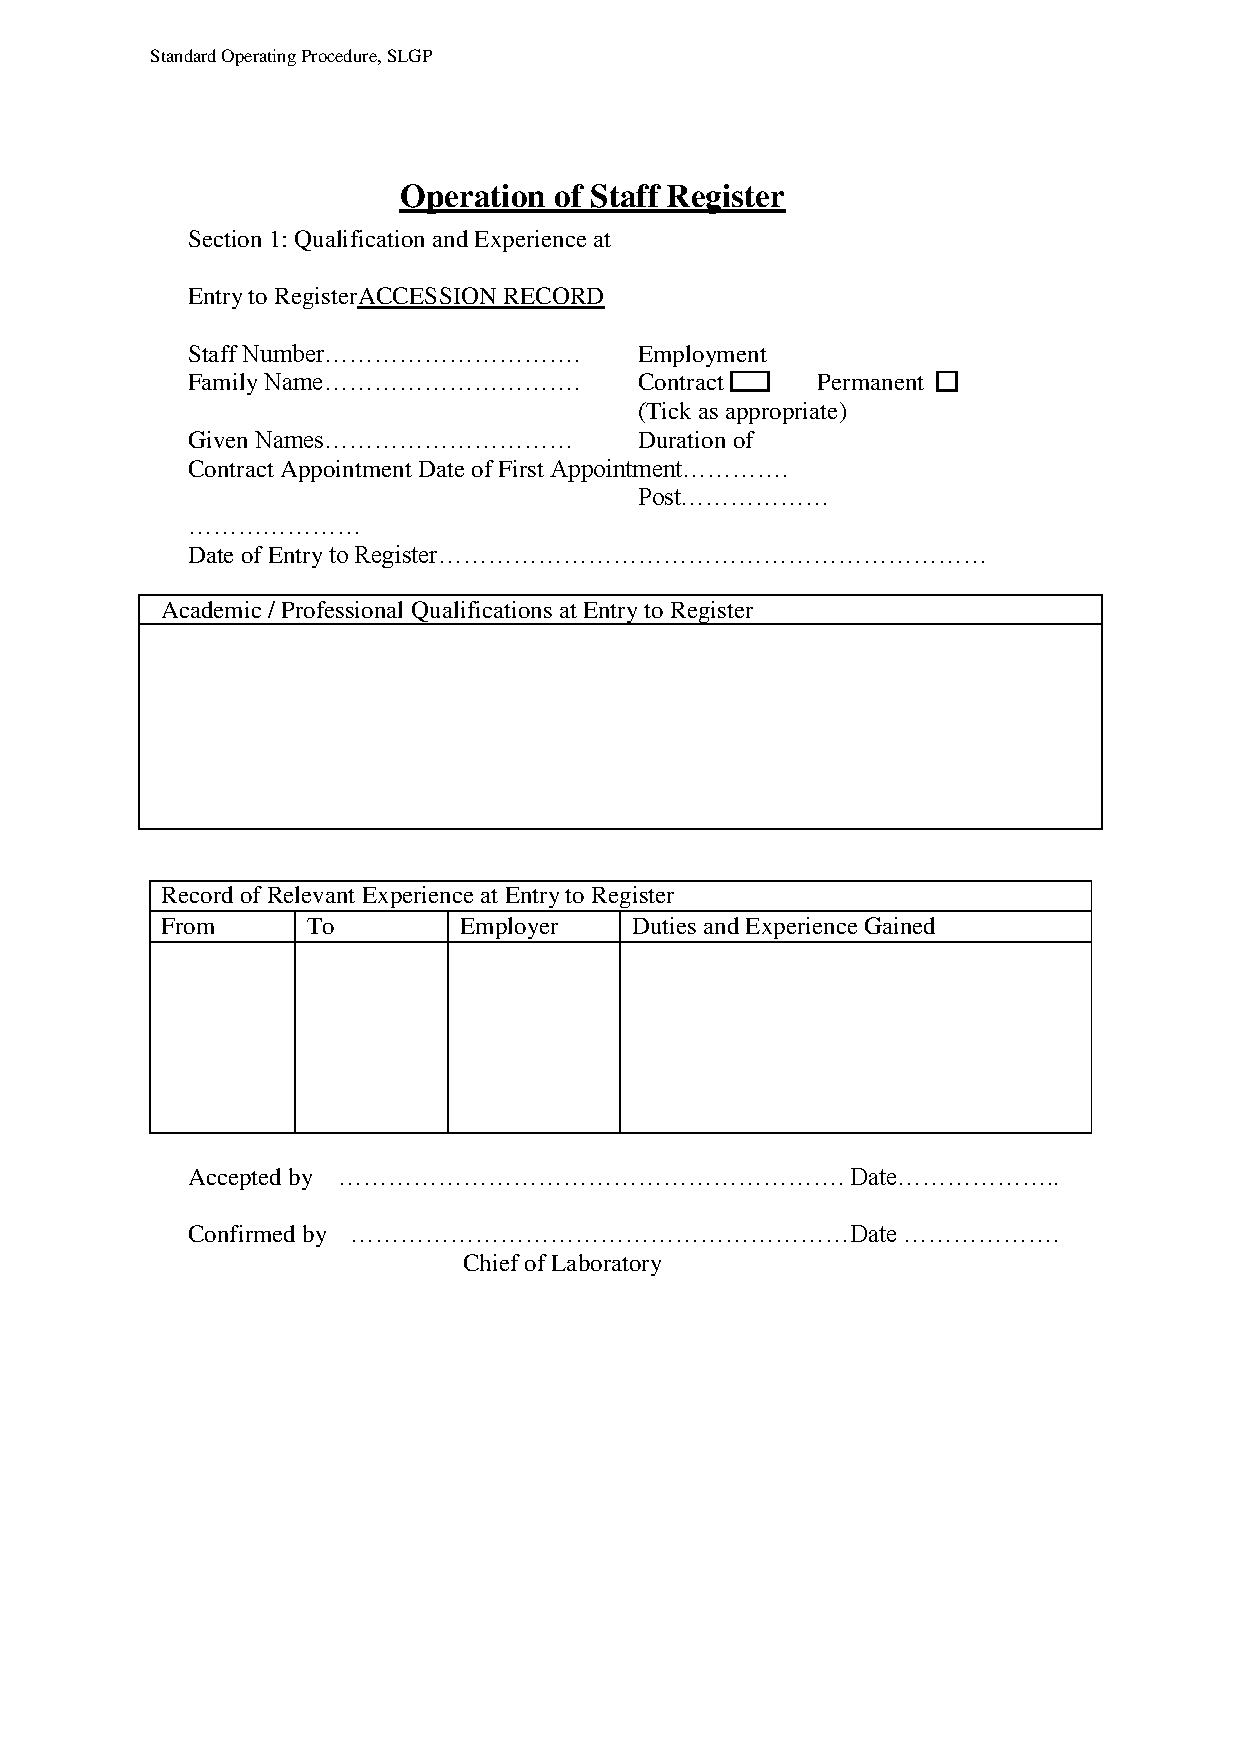
\includepdf[pages={-}]{extra/pro-forma-staff-register.pdf}

\chapter{Operation of staff register}\label{operation-of-staff-register}

\chapter{Operation and calibration of
blowers}\label{operation-and-calibration-of-blowers}

\section{Scope and Purposes}\label{scope-and-purposes}

\subsection{Scope}\label{scope-1}

\begin{itemize}
\tightlist
\item
  Blower's aids are often useful in seed testing laboratory to separate
  light weight material such as chaff and empty florets in grasses from
  the heavier seeds.
\end{itemize}

\subsection{Purpose}\label{purpose}

\begin{itemize}
\tightlist
\item
  Use of blowers saves at least 50 \% of the time spent on the purity
  test.
\end{itemize}

\section{Principle}\label{principle}

2.1 A good blower provides a uniform flow of air and is capable of
standardization as well as of retaining all the particles which it
separates.

\section{Operation Mechanism}\label{operation-mechanism}

\begin{itemize}
\tightlist
\item
  Blowing apparatus essentially consists of a centrifugal blower, the
  outlet of which is connected to the bottom end of a vertical tube of a
  few centimeters internal diameter and about half a meter length. A
  fine wire retains the sample before it is blown and also, holds the
  resultant heavy fraction. Different arrangements exist to catch the
  light fraction. A valve allows the wind velocity to be set a rate that
  has been found optimal for the kind of seed.
\item
  For certain species ISTA has devised an alternative - the Uniform
  Blowing Method. To this end ISTA Secretariat has distributed
  calibration samples and instructions to operate. The blower is set
  with the sample and after blowing the samples to be tested, the heavy
  fraction is considered to be full and the light fraction is considered
  to be empty. The method is compulsory for Poa pratensis and Dactylis
  glomerata and it is recommended for Chloris gayana as an alternative
  to the hand method.
\end{itemize}

\section{Calibration of the Blower}\label{calibration-of-the-blower}

\begin{itemize}
\tightlist
\item
  Carry out calibration of the blower using specially prepared samples
  of the relevant species in which the light and heavy fractions are
  distinctively stained.
\item
  Keep these samples normally in dust and moisture proof containers.
\item
  Regularly check the calibration of the blower as the setting will be
  affected by atmospheric pressure, humidity, temperature, draughts and
  even variations in electric voltage of power supply.
\item
  Analyst In-charge normally takes the responsibility of calibration of
  a blower and carries it out according to a strict procedure.
\end{itemize}

\chapter{Use and calibration of
balances}\label{use-and-calibration-of-balances}

\section{Scope and purposes}\label{scope-and-purposes-1}

\subsection{Scope}\label{scope-2}

\begin{itemize}
\tightlist
\item
  The essential piece of equipment for a seed analyst is a balance. The
  sample submitted for testing should contain sufficient seed in
  quantity and should be compatible to minimum sample weights for each
  kind of seed as specified in Seed Regulations. This situation demands
  a precision balance.
\item
  Purpose
\item
  This SOP 6 intends to give a general understanding on the basic kinds
  of balance available for seed analysis together with guidance on the
  use of these balances in general.
\end{itemize}

\section{Principle}\label{principle-1}

\begin{itemize}
\tightlist
\item
  Balances to be used in the laboratory must be checked for its
  performance each day that they are calibrated with the standard weight
  of the appropriate mass.
\end{itemize}

\section{Kinds of Balances}\label{kinds-of-balances}

\begin{itemize}
\tightlist
\item
  There are three basic kinds of balances in common usage. They are
  conveniently described as mechanical, electromechanical and
  electronic. If they are properly used, there should be no difference
  between them in quality of results.
\item
  Mechanical balances are the most basic type. They are true balances in
  that the object to be weighed is balanced against a fixed known mass.
  They require no electricity.
\item
  Electromechanical balance is an advanced form of the basic type. They
  do balance an object against a known mass but use a light and system
  of moving mirrors to indicate the weight on a moving scale. Counter
  weights are normally selected by turning one or more knobs connected
  to a system of levers, which release a series of weights in turn on to
  the balance beam. They are faster to use than mechanical balances, but
  the degree of precision and complication in their construction makes
  them expensive to build and they need regular skilled attention if
  accuracy is not to be deteriorated. This type of balance is being
  rapidly replaced by the electronic type.
\item
  In principle, Electronic type balance is entirely different from
  either mechanical or electromechanical types. The basic idea is quite
  simple. The balance pan is fixed to an electromagnetic core, around
  which are electric coils forming what is called a force motor. In very
  simple terms, what happens is that the weight of the sample tries to
  push the core down and this is resisted by the balance feeding more
  power into the coils to keep it in place. As the required power is
  proportional to the weight on the pan, it is possible for the
  electronic brain of the balance to measure the power and to display it
  in terms of the weight on the pan. Electronic balances have the
  advantages of being very quick and easy to use and they need no
  regular maintenance.
\end{itemize}

\section{Operating Procedure for
Calibration}\label{operating-procedure-for-calibration}

\begin{itemize}
\tightlist
\item
  The laboratory should be equipped with two standard weights for this
  purpose.
\item
  CSTL has one digit- two electronic balance, two digits -one electronic
  balance, three digit- one electronic balance and four digits -one
  electronic balance. One is of 20 grams for the analytical balance with
  torsion scale. Another is of 500 grams for the other balances that are
  used in the CSTL.
\item
  Keep these standard weights in a very safe place and handle them using
  the correct procedures to ensure that their mass remains accurate.
\item
  Always use forceps or a gloved hand while handling these weights.
\item
  Place the weight on top of a tarred piece of tissue paper or lens
  cloth on the balance pan
\item
  Determine the weights of these standards in the analytical balance as
  a check according to the need.
\item
  Record the results of these checks on a ``Balance Control Chart''
  (Appendix XVII)
\item
  The allowable range on this chart is \(\pm\) half the minimum
  significant reading required, for example, if the need were to weigh
  to the nearest gram then the allowable range would be \(\pm\)
  \SI{0.5}{\gram} and if the need were to weigh to \SI{0.01}{\gram} then
  the allowable range would be \(\pm\) \SI{0.005}{\gram}.
\item
  If a balance reading goes outside the allowable range, withdraw it
  from the service and send it for maintenance. Do not put it in use
  until it again gives satisfactory calibration readings. Detail
  procedure is given in working instruction.
\end{itemize}

\chapter{Use and calibration of
thermometer}\label{use-and-calibration-of-thermometer}

\section{Scope and Purpose}\label{scope-and-purpose-2}

\subsection{Scope}\label{scope-3}

\begin{itemize}
\tightlist
\item
  Environment (Temperature, Relative Humidity etc.) plays a vital role
  in different seed testing methods in the laboratory. The temperature
  provided by incubators, germination cabinets, room germinators,
  pre-chilling, pre-heating, constant temperature, alternate temperature
  etc. has crucial role in testing role in testing. Temperatures must be
  checked using thermometers that are properly calibrated and whereas
  the daily records of temperature checks have to be maintained.
\end{itemize}

\subsection{Purpose}\label{purpose-1}

\begin{itemize}
\tightlist
\item
  The purpose of calibration of thermometers is to take into
  consideration that the temperature provided by incubators, germination
  cabinets and room germinators must be within \(\pm\)
  \SI{20}{\celsius}. Pre-chilling and pre-heating should be carried out
  within a range of \SI{50}{\celsius} and the oven temperatures used in
  the determination of seed moisture contents should be carried out
  within a temperature range of \SI{30}{\celsius}.
\end{itemize}

\section{Principle}\label{principle-2}

\begin{itemize}
\tightlist
\item
  In all cases, temperatures should be as uniform as possible throughout
  the equipment and should not vary by more than half the range
  permitted for the mean.
\item
  Temperatures must be checked using thermometers that are calibrated
  and daily records of temperature checks must be maintained.
\end{itemize}

\section{Operating Procedure for
Calibration}\label{operating-procedure-for-calibration-1}

\begin{itemize}
\tightlist
\item
  Check the performance of temperature controlled equipment data logger.
\item
  Monitor the temperature of each piece of equipment over a period of at
  least seven days at half an hour intervals.
\item
  The temperature profiles of apparatus should then be derived by
  plating probes on top, middle and bottom shelves and at three
  positions on the middle shelf at the front, middle and back.
\item
  The temperature profile for any piece of apparatus should have a range
  of less than one half the range permitted for the mean temperature.
\item
  Temperature profiles can be derived over a period of 24 hours with
  readings taken at half hourly intervals.
\item
  During all temperature monitoring operations the apparatus should not
  be opened or otherwise disturbed.
\item
  Above-mentioned temperature monitoring exercise is repeated on an
  annual basis.
\item
  Records of temperature monitoring exercises are filed in the Equipment
  Register.
\item
  Apparatus is replaced if maintenance and adjustment fails to ensure
  that the temperature specifications are met.
\item
  For future orders of any temperature-controlled equipment, the
  required temperature specification should be quoted as a condition for
  the acceptance of the equipment.
\item
  The new equipment is installed and is used only after its temperature
  is monitored and profiles are derived.
\item
  Equipment that fails to meet the required specification is returned to
  the manufacturer and no payment is made.
\end{itemize}

\section{Monitoring Procedure}\label{monitoring-procedure}

\begin{itemize}
\tightlist
\item
  Temperature controlled items of equipment that are in service and
  conform to temperature specifications are routinely monitored.
\item
  When these are in use the temperature reading is recorded each day and
  is charted.
\item
  At least two readings are taken each day.
\item
  In the case of alternating temperature equipment, at least one reading
  is taken in the high temperature phase and one in the low temperature
  phase. An example of a temperature-monitoring chart that could be
  attached to an incubator is given in Appendix XVI. Completed
  temperature charts are filed in the Equipment Register. They are
  required of be retained for five years and be presented for inspection
  by auditors if required.
\item
  If the temperature of a piece of apparatus goes outside the required
  limits, it is withdrawn from the service.
\item
  Before accepting back to the service after any maintenance, the
  apparatus is checked as outlined above. Details of such checks are
  filed in the Equipment Register.
\item
  In freezers, temperature measurements are made with A20C/ Total
  Thermometer, which is a total immersion thermometer covering the range
  \SIrange{-20}{20}{\celsius} marked in \SI{0.1}{\celsius} intervals.
\item
  In Refrigerators, Incubators, Germinators and germination room, the
  temperature measurements are made with a calibrated A 40C/ Total
  Thermometer, which is a total immersion thermometer covering the range
  of \SIrange{0.5}{40.5}{\celsius} marked in \SI{0.1}{\celsius}
  intervals.
\item
  Thermometers for the above and freezers are placed in a clear glass
  tube (length: 431mm, OD: 14mm, ID: 12mm), which is then filled with
  glycerol and sealed at the open and with plastic film and adhesive
  tape. The tube containing the thermometer is placed as near the middle
  of the working area as possible avoiding newly introduced items that
  have not yet had time to reach the correct temperature. The tube is
  left in place for at least one hour and then a reading is taken as
  soon as the door is opened. The temperature is recorded and expressed
  to one decimal place.
\item
  Measurement in ovens and drying cabinets, which are provided with a
  port of insertion for the thermometer, is made with a partial
  immersion thermometer with 100mm immersion.
\item
  Care should be taken to site the thermometer so that the immersion
  length indication is just visible when it is viewed from inside the
  piece of equipment.
\item
  Appropriate thermometers are B60C/100 type. They are a partial
  immersion thermometer covering a range of \SIrange{0}{60}{\celsius}
  marked in \SI{20}{\celsius} intervals.
\item
  A B105 C/100 that is a partial immersion thermometer covering the
  range of \SIrange{45}{105}{\celsius} marked in \SI{0.2}{\celsius}
  intervals.
\item
  A 160C/100 is a partial immersion thermometer covering the range of
  \SIrange{99}{160}{\celsius} marked in \SI{0.2}{\celsius} intervals.
  The immersion length of all three types is 100 mm. The thermometer
  actually used should be the one that places the nominal temperature of
  the apparatus nearest the middle of the scale range.
\item
  The thermometer is placed as near as possible to the middle of the
  unit.
\item
  If the appliance has a transparent door, the thermometer readings
  should be taken through the door without opening it.
\item
  However, care should be taken to ensure that the thermometer can be
  read properly without distortion of the view by the door material.
\item
  The two consecutive readings must not differ by more that one scale
  division on the thermometer.
\item
  Thermometers in drying cabinets and ovens are positioned and left to
  equilibrate for at least five minutes before any reading is observed.
\item
  All thermometers are calibrated on an annual basis and a record of
  calibrations are filed for at least five years.
\item
  For thermometers with a 00 C marking, ice point temperature readings
  are required. Where the scale of the thermometer does not go through
  00 C, the thermometer is calibrated against a calibrated K type
  thermocouple attached to a portable temperature meter
\end{itemize}

\chapter{Seed registration system}\label{seed-registration-system}

\section{Scope and Purpose}\label{scope-and-purpose-3}

\begin{itemize}
\tightlist
\item
  The main task of sample reception in administration unit is to
  register the submitted samples as in Appendix XVII of SOP8, provide
  them with identification number, decide what kinds of tests are
  required, and to prepare working sheets (analysis forms) for each
  test.
\end{itemize}

\section{Procedure}\label{procedure-1}

\begin{itemize}
\tightlist
\item
  Most of the samples receipt in the laboratory is by post, through peon
  and through other personnel.
\item
  Place these samples in the incoming containers until they are
  registered. Verify, before unpacking the sample, which both the sample
  and test desired meet the conditions regarding identification,
  marking, sealing, packing and weight etc.
\item
  Depending on the type of sample, sometimes, irregularities may come
  across such as

  \begin{itemize}
  \tightlist
  \item
    The species or cultivars name on the request form is not the same as
    on the label of the sample.
  \item
    A moisture test has been requested but a special moisture test
    sample has not been submitted.
  \item
    Lot of time appears to be elapsed since the sample was drawn from
    the lot.
  \item
    Weight of the submitted sample was not adequate.
  \end{itemize}
\item
  Record such irregularities on the request form.
\item
  Ask the applicant or the sampler to provide additional information.
\item
  Record all relevant details on the form.
\item
  Enter the information on the sample slip as in Appendix XVIII 0f SOP8
  for reference in case of seriously damaged package and sent the sample
  back to the sender or sampler.
\item
  In other cases, communicate with the sender for required information
  immediately.
\item
  Do not enter the identity of the applicant or client in the analysis
  form in order to avoid the biasness of analyst in analytical
  performance.
\item
  Stamp dates of receipt and sample registration number in the analysis
  forms, the request form and in the label of the sample. (The use of a
  numbering machine and rubber stamp is recommended not only for
  numbering and for dating but also for other items that appear
  frequently such as code number and species name.)
\item
  Arrange safe storage of blank forms, rubber stamps, scissors, glue
  etc. and make them readily available for the use in the sample
  reception section.
\item
  Arrange enough space for temporary storage of incoming samples so as
  to leave working surfaces free for safe handling of each sample and
  the preparation of the appropriate document.
\end{itemize}

\chapter{Sample mixing, calibration of dividers and operation of seed
divider
register}\label{sample-mixing-calibration-of-dividers-and-operation-of-seed-divider-register}

\section{Scope and purpose}\label{scope-and-purpose-4}

\subsection{Scope}\label{scope-4}

\begin{itemize}
\item
  For all tests to be carried out in the Central Seed Testing Laboratory
  it is necessary to prepare representative sample of submitted seed lot
  for examination. To obtain such representative sample equipment called
  SEED DIVIDER is used.
\item
  Seed Dividers that are used to generate representative seed sample are
  required to be calibrated and be traceable to international standard.
\end{itemize}

\subsection{Purpose}\label{purpose-2}

The result of all seed tests are dependent on the seed sample that is on
test and the purpose of this procedure is to ensure

\begin{itemize}
\tightlist
\item
  That all seed dividers that are used in the CSTL are regularly checked
  to make it certain that they deliver representative sample of the
  submitted sample lot under examination within their performance
  capabilities and operational requirements.
\item
  Those seed dividers, which are used to obtain representative working
  sample, and the result of which are reported by the section on its
  test certificates, are traceable to international standard.
\item
  That trends in the performance of seed dividers are monitored to
  anticipate potential out of calibration situations.
\end{itemize}

\subsection{Safety}\label{safety}

\begin{itemize}
\tightlist
\item
  All those personnel who are engaged in seed analysis must wear a
  fastened laboratory coat.
\item
  Seed is mixed and divided mechanically in a room. If seed is dressed
  with chemical, if it is chemically treated, or if it is dusty, the
  operation is done in a ventilated cupboard with the dust extraction
  system switched on.
\item
  If seed is chemically dressed or treated, protection gloves and
  facemask must be worn during the mixing and dividing process.
\item
  The electrical integrity of all centrifugal dividers must be checked
  regularly.
\item
  Staff members, using seed dividers, must also bring to attention of
  the responsible person of any concerns they have about the safety of
  any procedures involving the use of any seed divider.
\end{itemize}

\section{Principle and Methodology}\label{principle-and-methodology}

\subsection{Principle}\label{principle-3}

\begin{itemize}
\tightlist
\item
  All seed dividers operate on the same principle although the
  mechanical methods used may be quite different. A seed sample is
  thoroughly mixed before being divided into two equal portions.
\item
  The weight of the working sample required is achieved by a succession
  of mixing and halving operations.
\end{itemize}

\section{Methodology}\label{methodology}

Seed dividers in operation are of three different design types such as
a) Centrifugal Divider (Gamet type divider), b) Boerner Divider and c)
Riffle Divider.

\begin{itemize}
\tightlist
\item
  \textbf{Boerner Divider} consists of a hopper, a cone with numerous
  ports closely spaced around its circumference. Alternate ports lead
  through ducts to a common outlet on one side, and the others lead
  similarly to an outlet on the opposite side. A valve or gate at the
  base of the hopper regulates the retention flow of the seed through
  outlets into the seed pan. This divider is convenient to handle but it
  is difficult to check for cleanliness. From time to time it needs to
  be opened and cleaned with the use of blower.
\item
  \textbf{Riffle Type Divider} (Multi-slot divider) has rectangular
  ports that are held in straight row in a frame with alternate ports
  leading to right and left. When the seed is poured evenly over the
  frame, it flows down the ports with half of it to each side.
\item
  \textbf{Gamet Type Divider} (Centrifugal): This divider makes use of
  centrifugal force to mix and scatter seeds over the dividing surface.
  In this divider, the seeds fall onto rapidly rotating disc, which
  throws half of it out to each side. This divider tends to give
  variable results, if it is not properly operated. Care should be taken
  that the divider is leveled by means of the adjustable foot knobs and
  sample is poured centrally into the hopper.
\end{itemize}

\section{Persons Responsible for
Action}\label{persons-responsible-for-action}

The Chief of the laboratory unit or the Manager who is responsible for:

\begin{itemize}
\tightlist
\item
  To make it certain that all seed dividers, purchased for the purpose,
  meet the criteria required for the intended application and that they
  are checked against those criteria before being placed in service.
\item
  To arrange for initial calibration, preventative maintenance,
  servicing and any necessary repairs.
\item
  To ensure that all new seed dividers are endorsed in the " Seed
  Divider Register" in Annex -- XIX and are removed from the register
  when withdrawn from service.
\item
  To provide suitable calibration samples to check the performance of
  seed dividers
\item
  To appoint ``Responsible Person'' in Appendix--XX and a deputy for
  seed dividers.
\item
  The Responsible persons are required to maintain a general watching in
  brief of seed dividers and to ensure that any concerns regarding their
  operation are acted upon.
\item
  They must maintain the Seed Divider Register. It is also to ensure
  that all required checks on seed dividers and any maintenance or
  repairs that were carried out are properly recorded.
\item
  The responsible persons take the charge to ensure that immediately
  after servicing of any seed divider for any reason a calibration
  sample is used to check performance of the unit and the result so
  obtained is recorded.
\item
  The Responsible Person should

  \begin{itemize}
  \tightlist
  \item
    Ensure that pro-forma of Section 2, 3 and 4 (see Appendix XXI, XXII,
    XXIII) are displayed near each seed divider.
  \item
    Replace fully completed Section 2, 3 and 4 forms timorously and
    number them numerically starting from one.
  \item
    Sign completed section 2, 3 and 4 forms and file them in the Seed
    Divider Register.
  \item
    File details of any maintenance or repairs in the Seed Divider
    Register.
  \end{itemize}
\item
  All Staff Members 3.3.1 The first person to use a seed divider on any
  given month is required to carry out the monthly calibration check on
  the Seed Divider and to record the results on the appropriate forms.
  Appendix XXI, XXII, XXIII3.3.2 All staff members are required to
  ensure that the seed divider, which they are using has had a monthly
  calibration check. They must also bring to the attention of the
  Responsible Person about the correct functioning of any seed divider.
\item
  All staff are responsible for ensuring tat they do not use any seed
  divider for species for which it is unsuitable.
\item
  Staff members using seed dividers are responsible for ensuring that
  they are clean and properly leveled before commencing mixing and
  dividing operations.
\item
  Concerned user takes responsibility of cleaning dividers after use and
  ensures that they are properly cleaned.
\end{itemize}

\section{Operation of the Seed Divider
Register}\label{operation-of-the-seed-divider-register}

\subsection{Copies of relevant pro-forma for compilation of the Seed
Divider Register. Chief of the laboratory unit holds the master
copy.}\label{copies-of-relevant-pro-forma-for-compilation-of-the-seed-divider-register.-chief-of-the-laboratory-unit-holds-the-master-copy.}

\begin{itemize}
\tightlist
\item
  Appointment of Responsible Persons
\item
  The chief of the laboratory unit chooses Responsible Person and the
  Deputy among the staff members who should be familiar with the
  operation of the full range of seed dividers that are in use in the
  section.
\item
  As a rule, the Responsible Person should be of at least a Seed Analyst
  grade.
\item
  Chief of the laboratory unit records Current Responsible Person and
  the Deputy in the Responsible Person Section of the Seed Divider
  Register and then initials the entry.
\item
  If somebody replaces the current Responsible Person else the chief of
  the laboratory unit cancels the previous appointment by completing the
  ``Date Replaced'' column and initials the change.
\item
  Once the Responsible Person has been appointed the chief of the
  laboratory unit hands over the Seed Divider Register into her/his
  custody.
\end{itemize}

\subsection{Entry of New Seed Dividers on the Register and Monthly
Calibration
checks.}\label{entry-of-new-seed-dividers-on-the-register-and-monthly-calibration-checks.}

\begin{itemize}
\tightlist
\item
  This is the responsibility of the chief of the laboratory unit and is
  subject to the same procedures for purchase and performance checks as
  other equipment.
\item
  The chief of laboratory initiates a register entry for the seed
  divider by adding it to the index of the seed divider register and
  completing the appropriate parts of pro-forma for section 1 of the
  Register.
\item
  The chief of laboratory unit specifies the calibration sample to be
  used and the range of accuracy in terms of precision of sample and
  component division.
\item
  The chief of laboratory unit specifies the calibration sample to be
  used and the range of accuracy in terms of precision of sample and
  component division.
\item
  Persons carrying out checks and calibrations of seed dividers records
  the weight of components to the nearest of 0.1 gram.
\item
  Responsible Person put his or her initial in Sections 2, 3 and 4 of
  the Seed Divider Register, which records the monthly checks of a Seed
  Divider. He or she also fills details of Seed Divider in the blank
  pro-forma for section 2, 3 and 4.
\item
  To obtain the monthly sample and component division value, the
  Responsible Person takes the weight of the appropriate calibration
  sample and records it in the ``Initial Weight Column''. (Section 4)
\end{itemize}

Section 2: - The Responsible Person enters the ``Allowed Range'' in
Section 2 of the Register. It should normally be \(\pm\) 5\% the
accuracy specified by the chief of the laboratory unit and defines the
range within which the sample division must fall to confirm that the
seed divider is still within the calibration range. - The graphical part
of Section 2 should have its scale defined. In general, the scale should
be set in such a way that the ``Allowed Range'' represents a
displacement of between 50\% and 75\% of full scale on the graph on
either side of the nominal setting. - The responsible person mixes and
divides the calibration sample into two portions e.g.~A and B using the
new seed divider and weighs two portions and records it in section 2. In
the meantime, addition of A and B is also recorded in the sheet.
Percentage of the total weight of portions A and B is calculated and is
recorded in the appropriate columns. The deviation of the percentage
portions A form 50\% on the chart is calculated. The Responsible Person
puts initials with date in each entry.

Section 3: - The calibration sample is a mixture of two components a)
seed and b) Admixture. The weight of one of the components ``the
admixture'' is less than 42\%. Both portions A and B are weighed and are
recorded. - For portion A the components are separated and weighed, the
weight is recorded. Same is repeated for portion B. - The ``calibration
sample'' part of the form is now completed by

???

\begin{itemize}
\tightlist
\item
  The percentage admixture in the calibration sample is now calculated
  and recorded.
\item
  The proportion admixture in both portion A and B is calculated as
\end{itemize}

???

The tolerance for component separation is checked against the table
given in this SOP 9. To check the tolerance, the percentage admixture in
the calibration sample is located in the tolerance table and the
percentage of the admixture found in the two portions compared to the
values in the table opposite the total admixture value. If the actual
percentage of the admixture values obtained is greater than the table
values, component division is out of the limits required. The entry
should now be dated and initialed.

Section 4:

All components are combined, weighed and returned to the calibration
sample container. The initial weight of the calibration sample and the
final weight after mixing, division and component separation are
recorded on the section 4 form. The `allowed weight change' is entered
in the section 4 of the Register. It will normally be +/- a value
specified by the Chief of the laboratory unit and defines the range
within which any change in weight at any division must fall. Values
falling within this range are indicative of the calibration process
having been carried out without any excess gain or loss in sample
weight.

The entry should now be dated and initialed.

\begin{itemize}
\tightlist
\item
  The Responsible Person presents Section 1 to the Chief of Laboratory
  Unit for scrutiny and signature and places Section2, 3 and 4 near to
  the seed divider in a plastic pocket
\item
  Provided that the Chief is satisfied, the new seed divider meets
  satisfactory performance criteria and has gone through correct
  calibration then she or he may accept it into the seed divider
  register by signing section 1.1 for the seed divider accepting it for
  service.
\item
  The completed forms for section 1 of the seed divider register must be
  added as a new part of the register relevant to seed divider and the
  seed divider must be added to the contents section of the register.
  This must be done by the chief of the laboratory unit who must put his
  initial in the new entry.
\item
  The Chief of Laboratory Unit then informs. The Responsible Person that
  the seed divider is now accepted for use.
\item
  The Responsible Person must now arrange for the seed divider to have a
  label affixed to it showing its number.
\end{itemize}

\section{Regular Calibration of Seed
Divider}\label{regular-calibration-of-seed-divider}

\subsection{Calibration Frequency}\label{calibration-frequency}

\begin{itemize}
\tightlist
\item
  Traceable Seed Dividers are calibrated monthly by the first person to
  use the divider within any given month.
\item
  A seed divider does not need to be checked in month if it is not used.
\item
  If a seed divider is returned to use after any kind of maintenance or
  repairs, under no circumstances it is placed for use without
  undergoing a calibration.
\end{itemize}

\subsection{Appropriate Calibration
Samples}\label{appropriate-calibration-samples}

\begin{itemize}
\tightlist
\item
  The Chief of Laboratory prepares calibration samples to be used for
  the S purpose of checking the operation of seed dividers.
\item
  They are composed of seeds of two species, one of whose presence is
  less than 42\% on weight basis means the portion of admixture weight.
\item
  The species of seed taken into use and the precise compositions are a
  matter of concern to the chief of the laboratory unit.
\item
  Calibration samples are labeled with a number and details of the type
  of seed dividers that are checked with.
\item
  The chief of the laboratory keeps a logbook, which details the weight
  and composition of each calibration sample he prepares.
\item
  The chief of the laboratory unit issues new calibration samples as and
  when required.
\end{itemize}

\subsection{Care of Calibration
Samples}\label{care-of-calibration-samples}

\begin{itemize}
\tightlist
\item
  Calibration samples are only removed from their containers for as long
  as it is necessary and are returned immediately after the use.
\item
  It is important that every effort is made to avoid unnecessary
  contamination and or loss of sample during the mixing, dividing and
  separation procedures.
\item
  The chief of laboratory is informed when the total weight of the
  calibration sample is less than

  \begin{itemize}
  \tightlist
  \item
    900 grams if it is to be used on centrifugal and Boerner Dividers.
  \item
    500 grams if it is to be used on the Riffle type divider.
  \end{itemize}
\end{itemize}

\subsection{Monthly Check Procedure}\label{monthly-check-procedure}

The procedure being used is described in Appendix-XXI, XXII, XXIII.

\subsection{Recording of Calibrations}\label{recording-of-calibrations}

\begin{itemize}
\tightlist
\item
  All calibrations and checks are recorded on appropriate
  pro-forma.5.5.2 The person carrying out the check puts on his or her
  initial on the entries on the forms. When a form is full it should be
  returned to the Responsible Person who will check it, enter the end
  date, and the sign and puts the new date before filling it in the Seed
  Divider Register under the appropriate Seed Divider.
\item
  The Responsible Person issues a new form having completed the header
  with the details of the seed divider and check parameters. The page
  number, the next in numerical sequence for that seed divider and the
  start date of the chart is also filled in.
\item
  A seed divider fails the test if the indicated value differs from the
  allowed range and / or the Allowed Weight change and/ or if component
  separation is out of tolerance with anticipated values.
\end{itemize}

\section{Action on Failure}\label{action-on-failure}

\begin{itemize}
\tightlist
\item
  In the event that any seed divider fails any calibration or any person
  suspects that it is not functioning correctly for any reason, then the
  concerned person immediately labels the seed divider as ``OUT OF
  CALIBERATION, DO NOT USE'' and informs the person responsible for seed
  dividers.
\item
  The responsible person will investigate. Should the fault be confirmed
  then the Responsible Person informs the Chief of Laboratory and the
  later will arrange for the necessary repairs and recalibration.
\item
  If the chief of Laboratory determines that this is possible after
  inspection, then he or she institutes checks on suspect data and also
  institutes a ``Quality Failure Report''
\item
  The quality Manager and the chief of Laboratory consult among each
  other after having investigated the situation and determines whether
  the exists to notify clients of possible problems with reported data
  resulting from the seed divider being out of calibration.
\end{itemize}

\chapter{Operation and maintenance of the seed reference
collection}\label{operation-and-maintenance-of-the-seed-reference-collection}

\section{Scope and Purpose}\label{scope-and-purpose-5}

\subsection{Scope}\label{scope-5}

1.1.1 This procedure applies to all seed reference collections that are
used in CSTL. It is narrated as follows.

1.1.2 Main seed Reference Collection. This is the Master Collection
containing seed specimens of different species. It is located in the
office of the Head of Section of CSTL and is used as a means of
identifying seed, which are not in either of the other collections and
verifying additions to other collections.

1.1.3 Purity Laboratory Seed Reference Collection. This collection
contains seed specimens of species likely to be encountered in the
purity laboratory. It is used as a means of identifying seeds, which are
not in the Seed Analyst's Seed Reference Collections.

1.1.4 Seed Analyst's individual Seed Reference Collection

1.1.5 These are the Seed Analyst's own Individual Seed Reference
Collections.

\subsection{Purpose}\label{purpose-3}

The purpose of this procedure is to ensure that

1.2.1 All identifications made on seeds found in the course of the
Purity and Determination of other Seeds by number Test are traceable to
reference seed samples.

1.2.2 All seed reference collections are maintained so as to ensure that
seed identification can be made accurately and efficiently.

\section{Principle}\label{principle-4}

In the purity tests and determination of other seed by number tests,
Seed Analysts are required to identify contaminant seeds that are
present in the sample lot. This collection of seeds is facilitated in
identification, which contains authentic samples of seeds of different
species.

\section{Persons Responsible for
Action}\label{persons-responsible-for-action-1}

\subsection{Head of Section}\label{head-of-section}

\begin{itemize}
\tightlist
\item
  The Head of Section is responsible for ensuring that the seed
  reference collections are maintained in such a way that seed
  identifications can be made accurately and efficiently.
\item
  The Head of Section is responsible for appointing ``Responsible
  Person'' and Deputy for the seed reference collections. In practice,
  they are usually the Laboratory Manager and the Senior Seed Analyst
  in-charge of the Purity Laboratory respectively. 3.2 Responsible
  Person
\item
  The Responsible Person and Deputy Responsible Person are recorded in
  the Responsible Person Record Sheet by the Head of Section who
  initials the entries and hold records in the file in Appendix XIV. If
  the appointments replace existing Responsible persons, the Head of
  Section cancels the previous appointment by completing the ``date
  replaced'' column and initialing the change.
\item
  The Responsible Persons are required to maintain a general watching
  brief on the Seed Reference Collections and to ensure that any
  concerns regarding their operation are acted upon.
\end{itemize}

\subsection{Seed Analyst}\label{seed-analyst}

\begin{itemize}
\tightlist
\item
  Seed Analysts are required to ensure that their individual Seed
  Reference Collections are maintained in such a way that
  identifications can be carried out accurately and efficiently.
\item
  Seed Analysts are to ensure that they refer any doubtful
  identifications to the Responsible Person or Deputy Responsible
  Person.
\end{itemize}

\section{Nomenclature and
Classification}\label{nomenclature-and-classification}

\begin{itemize}
\tightlist
\item
  The Linnaean binominal system of nomenclature is used for the
  collections of naming of seeds. For each species, a botanical or
  ``Latin'' name is used.
\item
  Classification can help greatly in the identification of unknown seeds
  and uses the following groupings starting from species as the basic
  unit.
\end{itemize}

Genus - A group of closely related species Family - A group of closely
related genera Order - A group of closely related families Class - A
group of closely related orders Phylum - A group of closely related
classes

\begin{itemize}
\tightlist
\item
  The particular names used for the species in each of the collections
  follow the ISTA ``List of Stabilized Names'' 6th edition, 2013.
\end{itemize}

\section{Main Seed Reference
Collection}\label{main-seed-reference-collection}

\subsection{Location and structures}\label{location-and-structures}

The main Seed Reference Collection is situated in the office of the Head
of Section.

The arrangement of The Main Seed Reference Collection is such that it is
convenient and easy to use. The seeds are filed by family first, then by
genus and then by species. Seeds from the same botanical family are
grouped together.

\subsection{Source and Authentication of
Seed}\label{source-and-authentication-of-seed}

In a seed reference collection, it is vital that all specimens are
correctly identified before they are included. Seeds contained in the
Main Seed Reference Collection have been obtained from botanical gardens
and gene banks throughout the different continents. These seeds have
been obtained from authentic sources and the identity of each species
guaranteed by the supplier.

\subsection{Containers and labels}\label{containers-and-labels}

Specimens are kept in clear glass tubes, plastic boxes or cellophane
packets. The genus and species' botanical names are either enclosed or
attached on a label along with the index reference number. Details of
the country and place of origin where available, are also noted on the
label.

When an Analyst finds a seed in an analysis with which she or he is
unfamiliar, she or he firstly refers to his/her own individual seed
reference collection. If no positive identification is made, the larger
purity laboratory reference collection is referred to. If he/ she is
still unable to identify the seed or seeds with the aid of these
collections, the Main Seed Reference Collection is then finally
referred.

\subsection{Maintenance}\label{maintenance}

Name changes take place in all areas of taxonomy. Botanical family
names, genus names and species names can be changed following work
completed by taxonomists. When this happens, the new names are listed in
ISTA publications such as the Newsletter or Updates to the ISTA List of
stabilized plant Names. It is then the job of the Responsible Person to
update the relevant family, genus or species names in the Main Seed
Reference Collection. The Responsible Person also has to ensure that
these name changes are carried out in the purity laboratory reference
collection and the Analyst's own individual seed reference collections
with verified references. This task is usually delegated to the Deputy
Responsible Person.

\chapter{Physical purity test}\label{physical-purity-test}

\chapter{Germination test}\label{germination-test}

\chapter{Determination of seed moisture
content}\label{determination-of-seed-moisture-content}

\chapter{Determination of other seed
number}\label{determination-of-other-seed-number}

\chapter{Determination of thousand seed
weight}\label{determination-of-thousand-seed-weight}

\chapter{Tetrazolium test}\label{tetrazolium-test}

\chapter{Variation in seed testing and the use of tolerances and limits
of
variation}\label{variation-in-seed-testing-and-the-use-of-tolerances-and-limits-of-variation}

\chapter{Production and control of
media}\label{production-and-control-of-media}

\chapter{Guard sample storage}\label{guard-sample-storage}

\chapter{Procedure for check on germination
substrate}\label{procedure-for-check-on-germination-substrate}

\chapter{Issuing of ISTA
certificates}\label{issuing-of-ista-certificates}

\chapter{Proficiency sample testing}\label{proficiency-sample-testing}

\bibliography{book.bib,packages.bib}

\end{document}
